\todo{Wichtige Begriffe erklären}

\subsection{pn-Übergang}
	\subsubsection{Grundverhalten}
	 	Ein PN-(Homo-)Übergang liegt vor, wenn zwei Halbleiter aus dem selben Material in Kontakt sind, deren Dotierung unterschiedlich ist. 
	 	\newline
	 	Im thermischen Gleichgewicht ohne externes Feld  	bleibt das Ferminiveau konstant (Pinning)
	 	\newline
	 	\begin{center}
	 		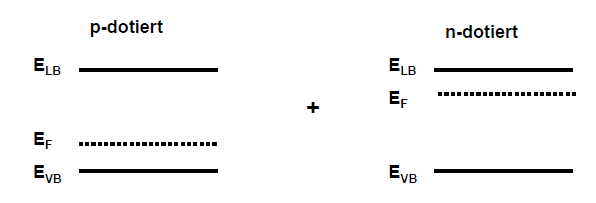
\includegraphics[width=0.6\linewidth]{Kapitel/Kap08/PN-uebergang_1.png}
		 	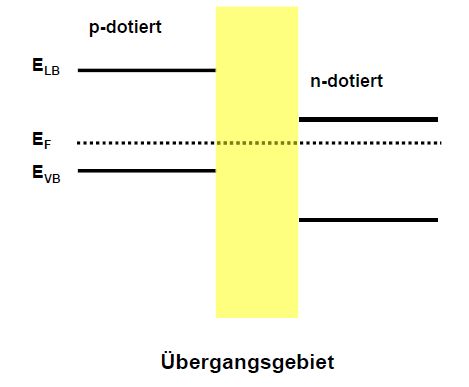
\includegraphics[width=0.35\linewidth]{Kapitel/Kap08/PN-uebergang_2.png}
		\end{center}
 	\subsubsection{metallurgische Grenze}
 		Der Punkt M, an dem die Dotierung sich von p zu n  	ändert, wird metallurgische Grenze genannt.
 		\begin{center}
 			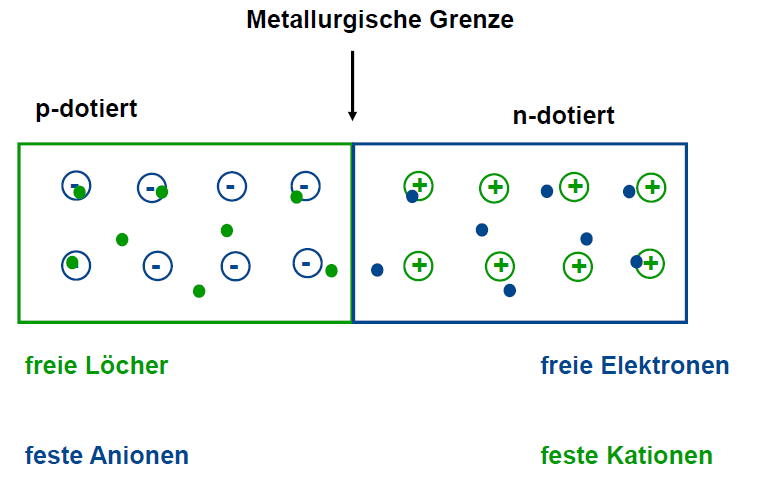
\includegraphics[width=0.4\linewidth]{Kapitel/Kap08/metallurgischeGrenze}
 		\end{center}
 		
 	\subsubsection{Diffusion und Drift}
 		\begin{enumerate}
 			\item Aufgrund des hohen Ladungsträgerkonzentrationsunterschiedes
 			kommt es zur Diffusion:
 			\begin{itemize}
 				\item von freien Löchern aus dem p-Gebiet ins n-Gebiet.
 				\item und von freien Elektronen aus dem n-Gebiet ins p-Gebiet
 			\end{itemize}
 			\item In der Nähe der Grenze M rekombinieren dann die diffundierten Ladungsträger mit den dortigen Majoritätsträgern.
 			\item Es kommt zu einer Verarmung der freien Ladungsträgern
 			\item Durch die verbleibenden festen Akzeptor-Ionen (p-Gebiet) und Donator-Ionen (n-Gebiet) entsteht ein lokales E-Feld entgegen der Diffusionsrichtung der Ladungsträger. Dies führt zu Driftströmen der freien Ladungsträgern.
 			\item Es stellt sich ein Gleichgewicht ein, so dass sich die Ladungsträgerströme resultierend aus Drift und Diffusion genau kompensieren.
 		\end{enumerate}
 		%drift und diffusion
		 \begin{center}
		 	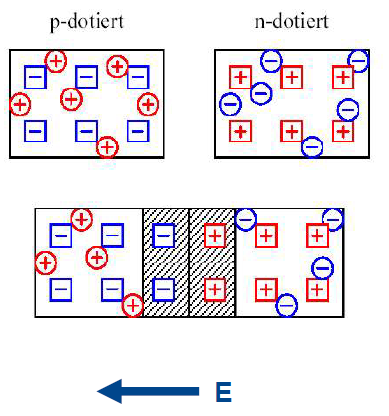
\includegraphics[width=0.4\linewidth]{Kapitel/Kap08/driftUndDiffusion}
		 \end{center}

	\subsubsection{Raumladungszone / Verarmungszone}
		Die Raumladungszone entsteht durch die Rekombination der freien Ladungsträger an der metallurigischen Grenze. Hierbei kommt es zur Verarmung der freien Ladungsträger, weshalb diese auch Veramungszone genannt wird. 
	\subsubsection{Eingebautes Feld}
	
		\begin{center}
			Zwischen den Festen Donator und Akzeptor-Ionen entsteht im Bereich der Raumladungszone ein elektrisches Feld.
			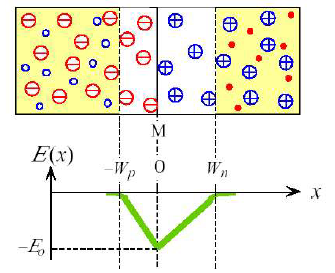
\includegraphics[width=0.4\linewidth]{Kapitel/Kap08/eingebautesFeld.png}
		\end{center}
		Den maximalen Wert $E_0$ des negativen elektrischen Feldes erreicht man an der Stelle der metallurgischen Grenze
		\newline
		Das elektrische Feld im thermischen Gleichgewicht wird eingebautes Feld genannt.
		
	\subsubsection{Diffusionsspannung}
		Die Spannung, die im thermischen Gleichgewicht über den pn-Übergang abfällt ($V_0$), wird auch 		eingebaute Spannung oder Diffusionsspannung ($U_D$) genannt.
		
		$V_0 = - \frac{E_0*W}{2}$
		
	\subsubsection{Breite der Raumladungszone}
		Die Breite der Raumladungszone hängt von den Donator- und Akzeptorkonzentrationen ab. Es gilt:			
		\begin{center}
			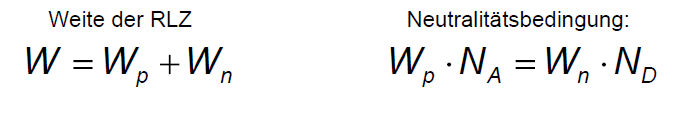
\includegraphics[width=0.5\linewidth]{Kapitel/Kap08/breiteRaumladungszoneNeutralisaetsbedingung.png}	
		\end{center}
	
		Daraus ergibt sich:	Für $N_A > N_D$ gilt $W_n > W_p$
		\newline
		Die Ausdehnung erfolgt immer stärker in das niedriger
		dotierte Gebiet.
		\newline
		Die Breite der Raumladungszone sinkt mit zunehmender Dotierung des n- bzw. p-Gebietes.
		\newline
		\textbf{Größenordnung Raumladungszone:}
		
		Annahme: Silizium mit p-Dotierung = n-Dotierung = $10^{18} cm^{-3}$
		
		Raumladungszone $W ca. 1 \mu m$
	
	\subsubsection{pn-Übergang mit externer Spannung}
	Externe Spannung V kann W vergrößern oder verkleinern:
	\begin{itemize}
		\item Für $V > V_0$ verschwindet die Raumladungszone -> Flussspannung 
		\item Für eine negative Spannung vergrößert sich die Raumladungszone -> Sperrspannung
	\end{itemize}
	\begin{center}
		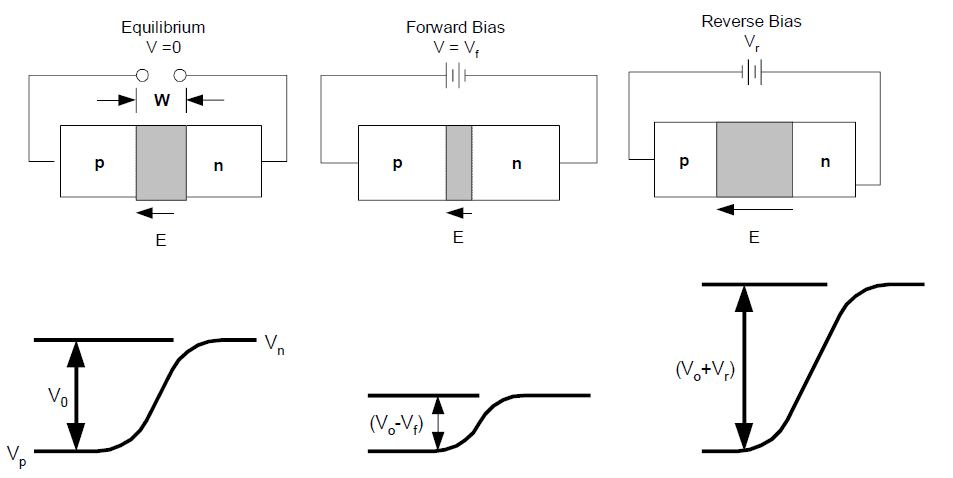
\includegraphics[width=0.6\linewidth]{Kapitel/Kap08/pnUebergangExterneSpannung}
	\end{center}
	\begin{center}
		Gleichgewicht, Flussrichtung, Sperrrichtung
	\end{center}
	
\subsection{pn-Diode}
	Bei einer pn-Diode treffen ein p und ein n-Gebiet aufeinander. Durch Ablegung einer Spannung kann die Diode den Strom leiten, da die Raumladungszone gegen Null geht.
	\begin{center}
		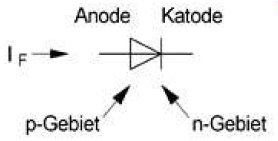
\includegraphics[width=0.3\linewidth]{Kapitel/Kap08/Diode}
	\end{center}

	\subsubsection{Kennlinien für verschiedene Halbleitermaterialien}
		Größere Bandlücke verschiebt das Einsetzen des Stromes zu höheren Spannungen.
		\begin{center}
			\centering
			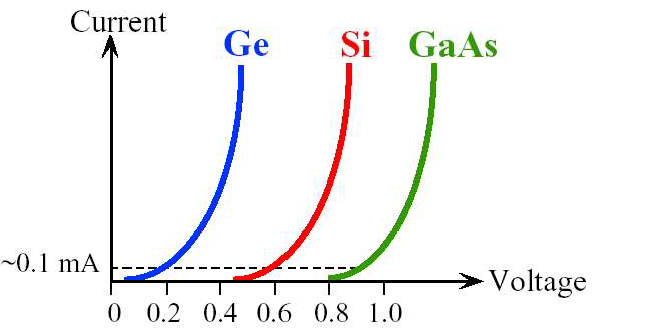
\includegraphics[width=0.7\linewidth]{Kapitel/Kap08/DiodeVerschiedeneHLMat.png}	
		\end{center}
	
	
	\subsubsection{Flusspolung, Sperrrichtung}
		\textbf{Flusspolung: }
		\begin{center}
			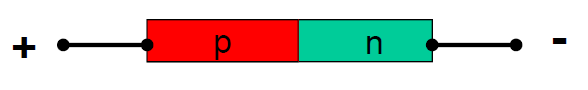
\includegraphics[width=0.5\linewidth]{Kapitel/Kap08/PNUebergangFlusspolung}
		\end{center}
		In Flussrichtung wird die Raumladungszone verringert und es kommt zu einem Stromfluss
		\newline
		\textbf{Sperrichtung:}
		\begin{center}
			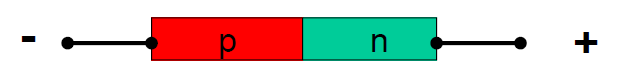
\includegraphics[width=0.5\linewidth]{Kapitel/Kap08/sperrichtung}
		\end{center}
		In Sperrichtung ist kein großer Strom aufrecht zu
		erhalten. Es entsteht trotzdem ein kleiner Strom (Sperrstrom), da Minoritätsträger
		in die Raumladungszone diffundieren und dann
		durch das elektrische Feld ins gegenüberliegende
		Gebiet transportiert werden.
		Der Sperrstrom kann noch weitere Bestandteile haben, z. B. Oberflächenleckströme
		
	\subsubsection{Ideale Diodengleichung}
		\begin{center}
			Ideale Dioden-Gleichung oder Shockley-Gleichung.
			Wichtig hierbei ist, dass der Strom proportional exponentiell von der Bandlücke des Materials abhängt.
			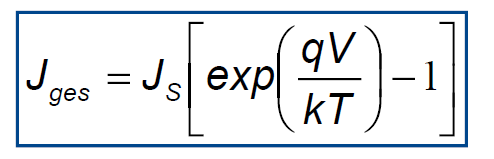
\includegraphics[width=0.3\linewidth]{Kapitel/Kap08/IdealeDiodengleichung.png}
			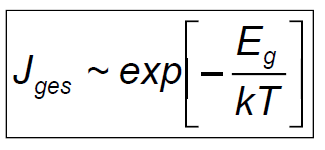
\includegraphics[width=0.2\linewidth]{Kapitel/Kap08/IdealeDiodengleichungProportionalitaet.png}	
		\end{center}
	
	\subsubsection{Ideal vs. Real}
		\begin{center}
			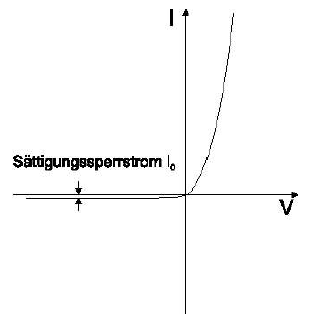
\includegraphics[width=0.25\linewidth]{Kapitel/Kap08/IdealvsReal.png}
			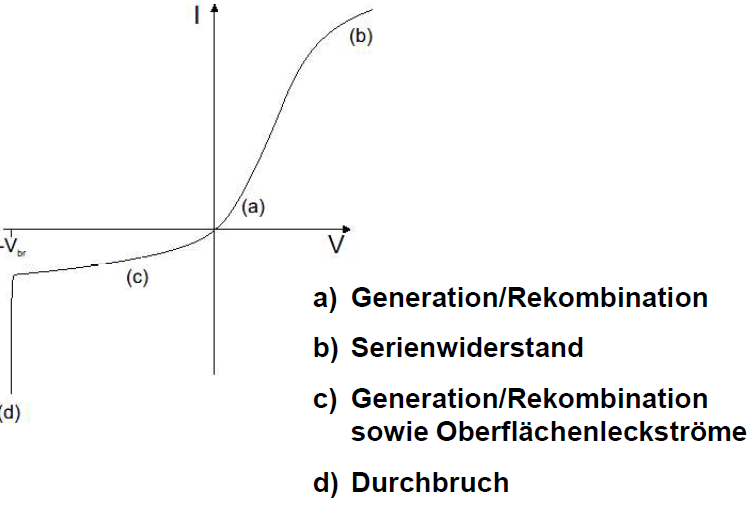
\includegraphics[width=0.35\linewidth]{Kapitel/Kap08/RealeDiode}
			
		\end{center}

	\subsubsection{Idealitätsfaktor}
		In realen pn-Übergängen tritt eine gewisse Rekombination in der Raumladungszone auf, was zu einem zusätzlichen äußeren Strom führt. 
		Gesamtstrom in einer pn-Diode ergibt sich daher aus der Summe des idealen Diodenstromes mit dem
		Rekombinationsstrom in der RLZ:
		\newline
		Bei der Beschreibung von realen Diodencharakteristiken in bestimmten Spannungsbereichen wird dabei folgende Gleichung verwendet (Gleichung irrelevant)
		\begin{center}
			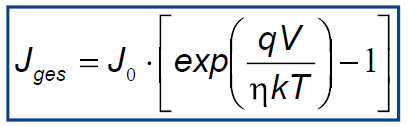
\includegraphics[width=0.3\linewidth]{Kapitel/Kap08/genaherteGleichung}
		\end{center}
		Der darin enthaltene \textbf{ Faktor $\eta$ wird als Idealitätsfaktor bezeichnet und liegt immer zwischen 1 und 2}
		\begin{center}
			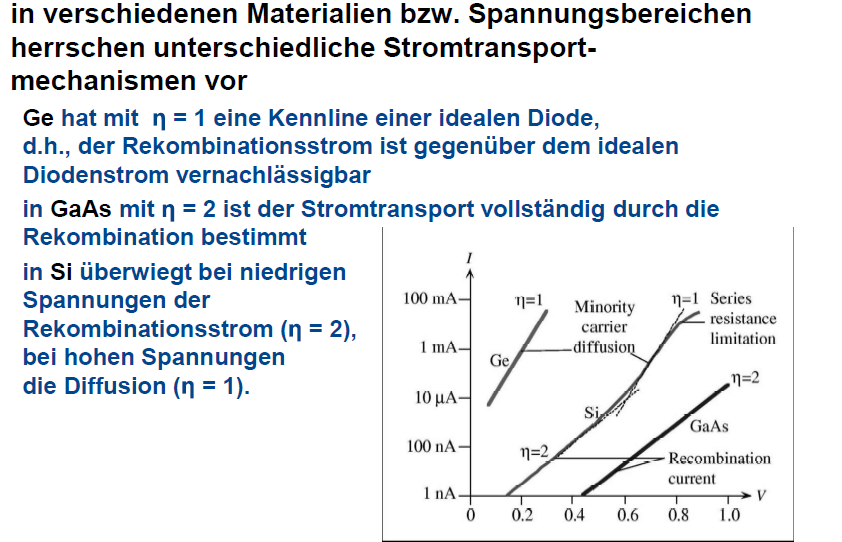
\includegraphics[width=0.5\linewidth]{Kapitel/Kap08/IdealitaetsfaktorBeispiel}
		\end{center}
		
	\subsubsection{Temperaturabhängigkeiten}
		Bei wachsender Temperatur nimmt der ideale
		Stromanteil gegenüber dem nichtidealen zu. Die Einsatzspannung der Diode sinkt.
		\begin{center}
			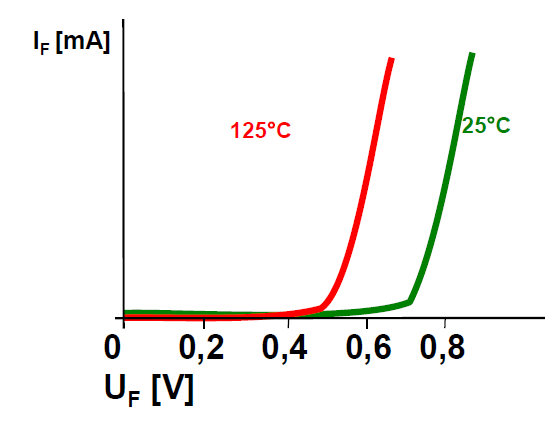
\includegraphics[width=0.25\linewidth]{Kapitel/Kap08/temperaturabhaengigkeit1}
		\end{center}
		Mit wachsender Temperatur nimmt auch der Sperrstrom zu
		\begin{center}
			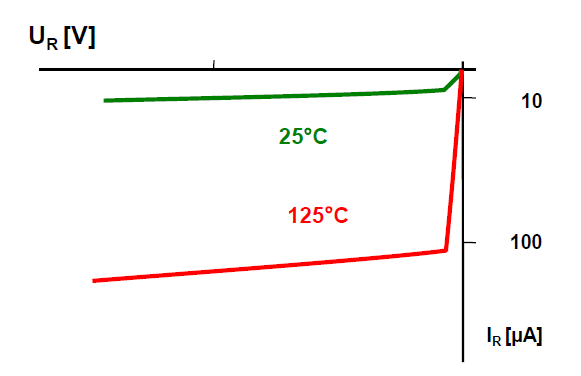
\includegraphics[width=0.25\linewidth]{Kapitel/Kap08/temperaturabhaengigkeit2}
		\end{center}
		
	
	\subsubsection{Durchbruch}
	Die pn-Diode kann nicht mit beliebig großer Spannung in Sperrichtung betrieben werden.
	Eine zu hohe Spannung in Sperrichtung führt dazu, dass die Diode "durchbricht". Der Strom steigt ab einer kritischen Sperrspannung (Durchbruchsspanung) sehr stark an. 
	\subsubsection{Lawinendurchbruch}
	Durch ausreichend hohe Sperrspannungen ist es 	möglich, die Raumladungszone und damit das 	elektrische Feld am pn- Übergang soweit zu vergrößern, 	dass die beschleunigten Ladungsträger ausreichend hohe Energien erreichen, um ihrerseits durch Stöße mit Kristallatomen weitere Elektron-Loch-Paare zu erzeugen (Stoßionisation).
	Die so generierten Elektronen und Löcher können bei ausreichender Beschleunigung im elektrischen Feld ihrerseits wieder Stoßionisationprozesse auszulösen.
	Somit kommt es zu einer Lawinenartigen Bildung von Ladungsträgern, der Sogenannte Lawinendurchbruch.
	\subsubsection{Zener-Effekt/-Diode}
	Der Zener-Effekt tritt bei hoch
	dotierten pn-Übergängen auf, in denen schmale Raumladungszonen und hohe elektrische Feldstärken auftreten.
	In diesem Fall kann es unter Sperrspannung zum Tunneln von Elektronen des Valenzbandes der p-Seite ins Leitungsband der n-Seite kommen, wobei auch Elektron-Lochpaare in der RLZ geschaffen werden. Dies führt zu einem Starken Anstieg des Stroms. Die kritische Spannung liegt dabei niedriger als die Durchbruchsspannung. 
	\newline
	Die auf diesem Effekt basierende Z-Dioden erlaubt es, dass sie in zahlreichen Schaltungen zur Stabilisierung und
	Begrenzung von elektrischen Spannungen eingesetzt werden.
	\begin{center}
		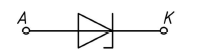
\includegraphics[width=0.3\linewidth]{Kapitel/Kap08/Zenerdiode}
	\end{center}
	
	\subsubsection{Varaktordioden}
		In Sperrrichtung wirkt die Sperrschicht bzw. Raumladungszone am pn-Übergang wie eine Kapazität.
		Ändert sich die Spannung an der Diode ändert sich auch die Kapazität der Sperrschicht.
		Die Varaktordiode wird daher als spannungsabhängige Kapazität (Varaktor) genutzt.
		Hierbei ist die Sperrschicht-Kapazität
		besonders groß. Dadurch sind große Kapazitätsänderungen möglich.
		\begin{center}
			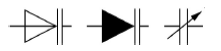
\includegraphics[width=0.3\linewidth]{Kapitel/Kap08/Varaktordiode}
		\end{center}
		
	
	\subsubsection{Diodentypen und ihre Anwendungsfelder}
		Vermutlich eher unwichtig:
		\begin{itemize}
			\item Optik -> Laserdiode, Fotodiode, LED
			\item Kapazitive Dioden
			\item Gesteuerte Gleichrichter und verwandte Bauelemente -> Vierschichtdioden, Thyristor
			\item diverse weitere
		\end{itemize}


\todo{Fragen aus Own Clowd zuordnen}
\todo{Gruppenübungs-Inhalte ergänzen}